\section{Evaluarea WTE}

Pentru a evalua simulatorul propus în această lucrare, au fost considerate patru caracteristici pentru a fi măsurate: puterea de procesare pe care simulatorul o folosește, procentul de \textit{memorie cu acces aleator} - \gls{ram} necesar funcţionării acestuia, timpul de iniţializare a simulatorului și spaţiul de stocare ocupat pe disc de \gls{wte}. Metoda de măsurare a acestor caracteristici și rezultatele acestora vor fi prezentate în paragrafele următoare.

\subsection{Metodologie}

Pentru a putea măsura cele patru caracteristici menţionate anterior, a fost nevoie de dezvoltarea unor soluții în simulator. Acestea au fost implementate în nucleul \gls{wte}.

Măsurarea timpului de iniţializare a simulatorului, a constat în folosirea unui cronometru oferit de limbajul Python. Acesta a fost pornit după citirea fişierelor de configurare și oprit după ce toate elementele topologiei simulate au fost create, înainte de pornirea interfeţei prin linie de comandă. Timpul astfel măsurat reprezintă durata de iniţializare a simulatorului și este exprimat în secunde, cu o precizie de trei zecimale. Valoarea acestuia a fost tipărită în consola simulatorului.

O abordare similară a fost folosită și în determinarea spațiului de stocare pe disc folosit de \gls{wte}. Înainte de începerea inițializării simulatorului se interoghează sistemul de operare asupra spațiului liber de pe disc. După terminarea inițializării se face o nouă interogare, diferenţa dintre aceste două valori reprezentând spaţiul pe disc ocupat de topologia simulată. Este ocupat și spațiu pe disc, nu doar în memoria \gls{ram} din cauza abordării folosite în utilitarul \textit{docker}, în care fiecare container are nevoie de spațiu pentru a-și reprezenta sistemul de fişiere din interior. Valoarea calculată este exprimată în MB și este afişată de asemenea în consola simulatorului, după terminarea inițializării.

Procentul memoriei cu acces aleator utilizat de simulator este dat, în cea mai mare parte, de către memoria necesară containerelor \textit{docker} asociate fiecărui element de rețea. Nucleul \gls{wte}, în calcularea acestui procent, neglijează alte valori (de exemplu chiar acest nucleu folosește la rândul său memorie cu acces aleator, care nu este însă semnificativă în comparaţie cu celelalte valori) și se bazează
doar pe valorile asociate containerelor \textit{docker}. În interfaţa prin linie de comandă a simulatorului a fost implementată o comandă care să calculeze acest procent. Calculul folosește informaţiile furnizate de o comandă a utilitarului \textit{docker}: \textit{docker stats}. Aceasta afişează procentul de memorie cu acces aleator utilizat de fiecare container care rulează. Implementarea comenzii din nucleul \gls{wte} va aduna aceste valori și va afişa pe ecran suma. Valoarea tipărită pe ecran reprezintă procentul de memorie cu acces aleator folosit pentru simularea topologiei de rețea.

Calcularea puterii de procesare a \gls{wte} se face prin aceeaşi comandă care afişează și procentul de memorie cu acces aleator folosit. Implementarea acesteia utilizează, de asemenea, comanda \textit{docker stats} oferită de utilitarul \textit{docker}, însă abordarea este puţin diferită. Diferenţa este dată de faptul că puterea de procesare nu este folosită în mod continuu de către containerele \textit{docker} asociate elementelor de rețea simulate. Astfel, dacă în momentul interogării sistemului de operare, unor containere nu le erau alocate cuante de timp de procesare, acestea apar cu zero procent de utilizare a procesorului. La o interogare ulterioară, acest procent ar putea fi altfel distribuit dispozitivelor simulate. Pentru ca valoarea măsurată să fie relevantă, a fost ales un număr de zece eşantioane pentru fiecare element de rețea simulat, procentul de putere de procesare asociat fiind reprezentat de media aritmetică a acestora. În mod empiric a fost observat că dacă s-ar fi ales un număr mai mare de eşantioane, de exemplu o sută, diferenţa valorii procentului final calculat ar fi fost foarte mică față de cazul celor zece eşantioane. Astfel, pentru a nu prelungi inutil timpul de calcul al acestui procent, s-a rămas la abordarea cu zece eşantioane. De asemenea, acest procent al puterii de procesare oferit de comanda \textit{docker stats} este raportat la un singur nucleu al procesorului, astfel încât în condiţii de utilizare intensă am fi putut avea valori ale procentului mai mari de 100\%. Din acest motiv, valoarea procentuală raportată a fost împărţită la numărul de nuclee ale procesorului. Pe scurt, procentul puterii de procesare se calculează astfel: se interoghează sistemul de operare prin comanda \textit{docker stats} asupra procentului folosit de fiecare container în parte și se face suma acestora. Acest lucru se repetă de zece ori (numărul de eşantioane considerat) și apoi se face media aritmetică. Valoarea astfel obţinută se împarte la numărul de nuclee ale procesorului, obţinând astfel valoarea finală a procentului de putere de procesare utilizată de simularea topologiei de rețea, care este afişată pe ecran.

Puterea de procesare și procentul de memorie cu acces aleator utilizate de către \gls{wte} au fost măsurate doar după ce dispozitivele simulate au fost înregistrate la echipamentul de control \gls{sdn}, stabilindu-se astfel conexiunile \gls{netconf} din rețea.

Toţi parametrii care au fost menţionaţi anterior au fost măsuraţi în diferite topologii tipice pentru rețelele de transport de date fără fir: topologii de tip inel (\textit{ring}), de tip arbore (\textit{tree}) sau de tip plasă (\textit{mesh}). Exemple de astfel de topologii, împreună cu detaliile dispozitivelor de rețea simulate în fiecare caz sunt ilustrate în Figurile~\ref{fig:topologies_ring}, \ref{fig:topologies_tree} și \ref{fig:topologies_mesh}.

\begin{figure}[h]
	\centering
	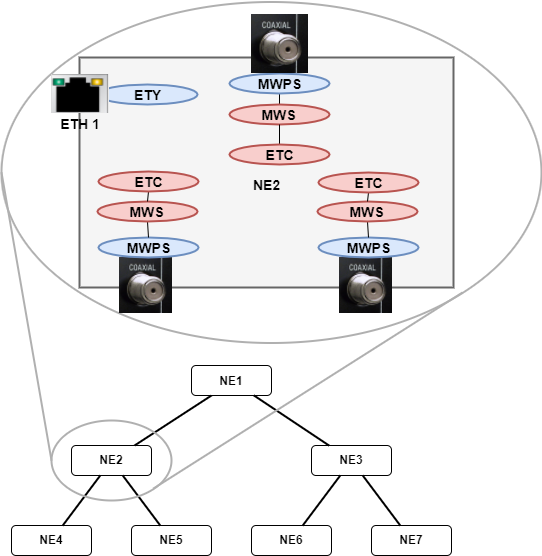
\includegraphics[width=0.6\textwidth]{topologies_tree}
	\caption{Topologie de rețea arbore, exemplu pentru 7 elemente simulate}
	\label{fig:topologies_tree}
\end{figure}

\begin{figure}[h]
	\centering
	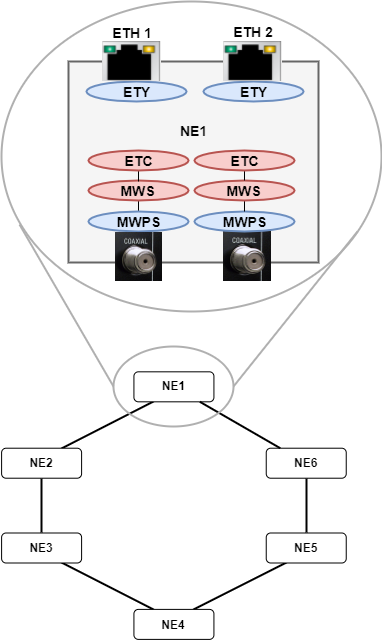
\includegraphics[width=0.6\textwidth]{topologies_ring}
	\caption{Topologie de rețea inel, exemplu pentru 6 elemente simulate}
	\label{fig:topologies_ring}
\end{figure}

\begin{figure}[h]
	\centering
	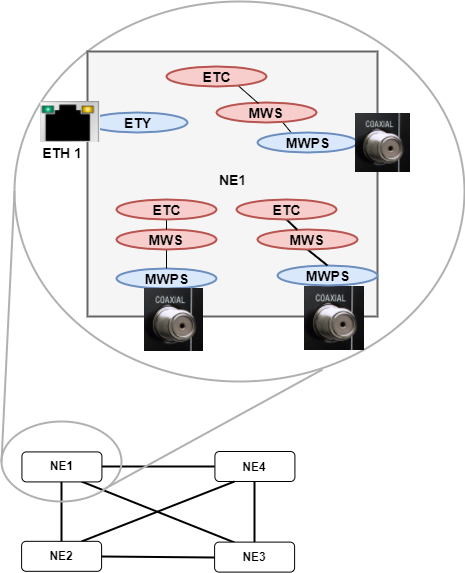
\includegraphics[width=0.6\textwidth]{topologies_mesh}
	\caption{Topologie de rețea plasă, exemplu pentru 4 elemente simulate}
	\label{fig:topologies_mesh}
\end{figure}

În cazul rețelelor de tip inel, au fost simulate topologii având un număr de elemente simulate de la 10 la 200, acesta crescând din 10 în 10. În această situaţie, un dispozitiv simulat are nevoie de două interfețe fără fir, reprezentate în modelele propuse de \gls{onf} prin obiecte de tip \gls{mwps}, pentru conexiunile cu vecinii. Fiecare astfel de interfață va avea și obiecte de tip \gls{mws} și \gls{etc} asociate. A fost aleasă și asocierea a două interfețe Ethernet fiecărui dispozitiv simulat, pentru a putea injecta trafic în nodul respectiv, reprezentată de obiecte de tip \gls{ety}. Astfel, fiecare dispozitiv simulat prezintă un număr de opt obiecte, care sunt reprezentate în containerul \textit{docker} asociat prin opt interfețe Linux.

Topologiile de tip arbore alese pentru simulare în cadrul evaluării au fost reprezentate de arbori binari. În acest caz, fiecare dispozitiv de rețea a avut nevoie de trei interfețe fără fir (una pentru conexiunea dinspre rădăcină și două pentru legăturile dinspre frunze), reprezentate prin obiecte de tip \gls{mwps}. Fiecare astfel de interfețe au asociate și obiectele de tip \gls{mws} și \gls{etc}. Fiecare element de rețea simulat a avut asociată și o interfață de tip Ethernet prin care să se poată injecta trafic, reprezentată de un element de tip \gls{ety}. În acest mod fiecare container \textit{docker} asociat a avut nevoie de zece interfețe Linux pentru reprezentarea internă a acestor obiecte. În simulările asociate evaluării au fost folosite topologii în care a fost variată adâncimea arborelui, de la 3 (însemnând un număr de 7 elemente de rețea), până la 7 (127 de dispozitive simulate).

Topologiile de tip plasă cu redundanţă maximă diferă de celelalte prin faptul că numărul total de interfețe simulate nu mai creşte liniar, ca în cazurile anterioare, ci pătratic cu numărul de elemente de rețea. Pentru o topologie de tip plasă cu $ N $ elemente de rețea vom avea un număr total de interfețe simulate de $ N(N-1) $ și respectiv $ N(N-1)/2 $ legături de date. Astfel, pentru \textit{N} elemente, fiecare dispozitiv simulat prezintă \textit{N-1} obiecte de tip \gls{mwps} pentru conexiunile dintre echipamente, respectiv \textit{N-1} obiecte de tip \gls{mws} și \textit{N-1} obiecte \gls{etc}. Fiecare astfel de dispozitiv are asociată și o interfață Ethernet (un obiect \gls{ety}), pentru injectarea de trafic.

Măsurătorile pentru evaluare au fost efectuate în trei medii diferite în care a fost instalat simulatorul \gls{wte}: local, pe un laptop cu o mașină virtuală Linux și în două medii de tip \textit{cloud}. Primul mediu \textit{cloud}, denumit Orbit \cite{orbitpage}, a fost pus la dispoziţie de compania AT\&T. Cel de-al doilea mediu este cel folosit în cea de-a patra demonstraţie de concept \gls{onf} și a fost asigurat de Deutsche Telekom (DT). Caracteristicile, precum și resursele de care dispune fiecare dintre aceste sisteme sunt reprezentate în Tabelul~\ref{tab:resources}.

\begin{table}[h]
	
	\caption{Caracteristicile sistemelor pe care s-a făcut evaluarea WTE.\label{tab:resources}}
	\begin{tabular}{|M{0.25\textwidth}|M{0.2\textwidth}|M{0.2\textwidth}|M{0.2\textwidth}|}
		\hline
		\textbf{Caracteristica} & \textbf{\emph{Mașina locală}} & \textbf{\emph{Orbit Cloud}} & \textbf{\emph{DT Cloud}} \tabularnewline
		\hline 
		Sistemul de operare & Linux & Linux & Linux \tabularnewline
		\hline 
		Versiunea de kernel & 4.4.0-93-generic & 4.4.0-83-generic & 4.4.0-89-generic
		\tabularnewline
		\hline 
		Arhitectura procesorului & x86\_64 & x86\_64 & x86\_64 \tabularnewline
		\hline 
		Memoria cu acces aleator & 4096 MB & 8 GB & 8GB \tabularnewline
		\hline 
		Capacitatea de stocare a discului & 32 GB & 80 GB & 80 GB \tabularnewline
		\hline 
		Frecvenţa procesorului & 2591.59 MHz & 2 GHz & 2500 MHz \tabularnewline
		\hline 
		Nuclee procesor & 4 & 4 & 4 \tabularnewline
		\hline \end{tabular}
\end{table}

%\subsection{Rezultatele măsurătorilor}

\subsection{Timpul de inițializare a simulatorului}

Prima caracteristică măsurată în procesul de evaluare a fost timpul de iniţializare a simulatorului. Acesta reprezintă durata de când simulatorul \gls{wte} este pornit, până când toate elementele rețelei (dispozitive, interfețe ale acestora și legăturile dintre ele) au fost adăugate în mediul de simulare și interfaţa prin linie de comandă este accesibilă. Figura~\ref{fig:boot_vs_ne_ring_v1} prezintă variaţia timpului de iniţializare cu numărul de elemente de rețea simulate, în cazul unei topologii de tip inel. Din cauza faptului că maşina locală are doar 4 GB de memorie cu acces aleator, simularea în acest mediu se opreşte la 130 de dispozitive simulate. În Figura~\ref{fig:boot_vs_ne_tree_v1} este ilustrată aceeaşi variaţie, în cazul simulării unei topologii de tip arbore, în timp ce Figura~\ref{fig:boot_vs_ne_mesh_v1} este folosită pentru a descrie cazul topologiei de tip plasă. Acestea arată o dependenţă liniară (aproximativ) între numărul de dispozitive simulate și timpul de iniţializare. 

\begin{figure}[hp]
	\centering
	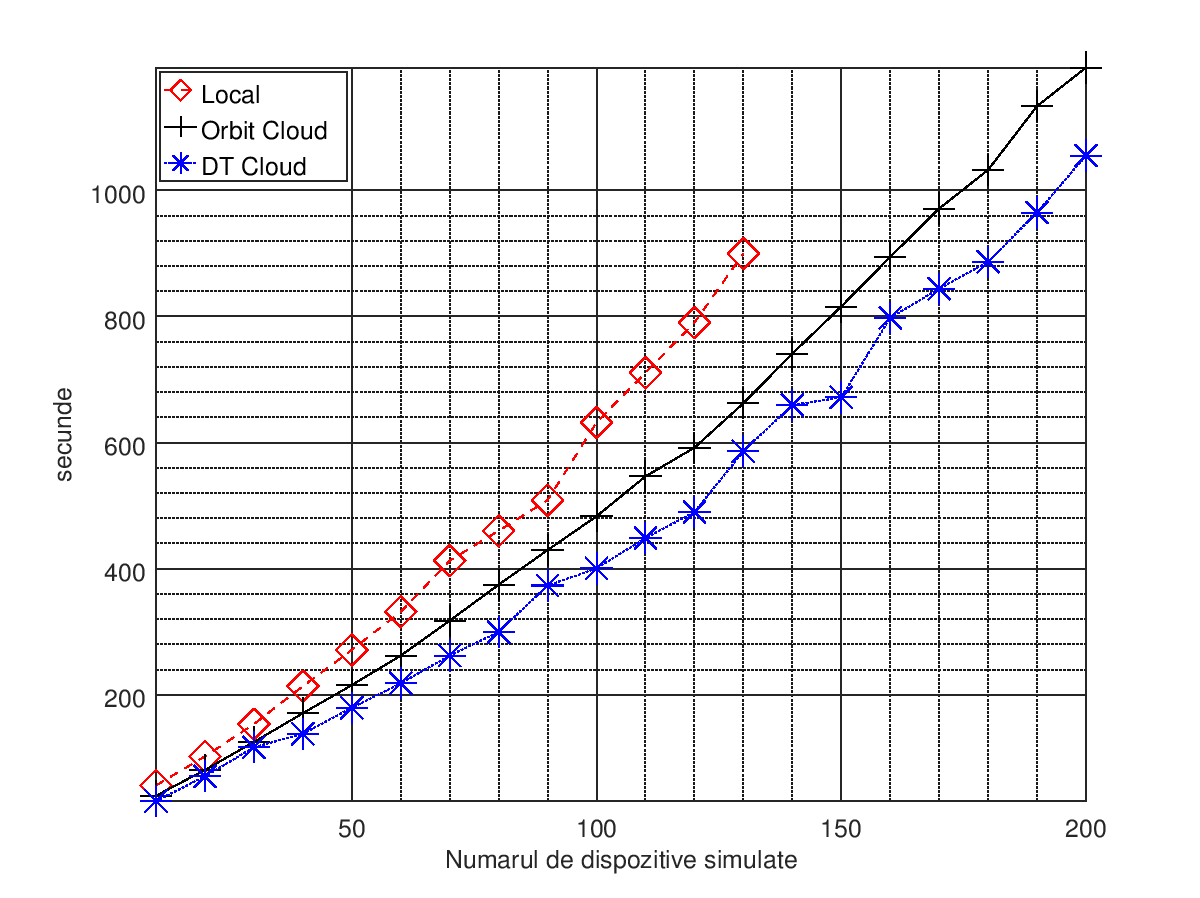
\includegraphics[width=0.85\textwidth]{boot_vs_ne_ring_v1}
	\caption{Timpul de iniţializare în funcție de numărul de dispozitive de rețea simulate, într-o rețea de tip \textbf{inel}}
	\label{fig:boot_vs_ne_ring_v1}
\end{figure}

\begin{figure}[hp]
	\centering
	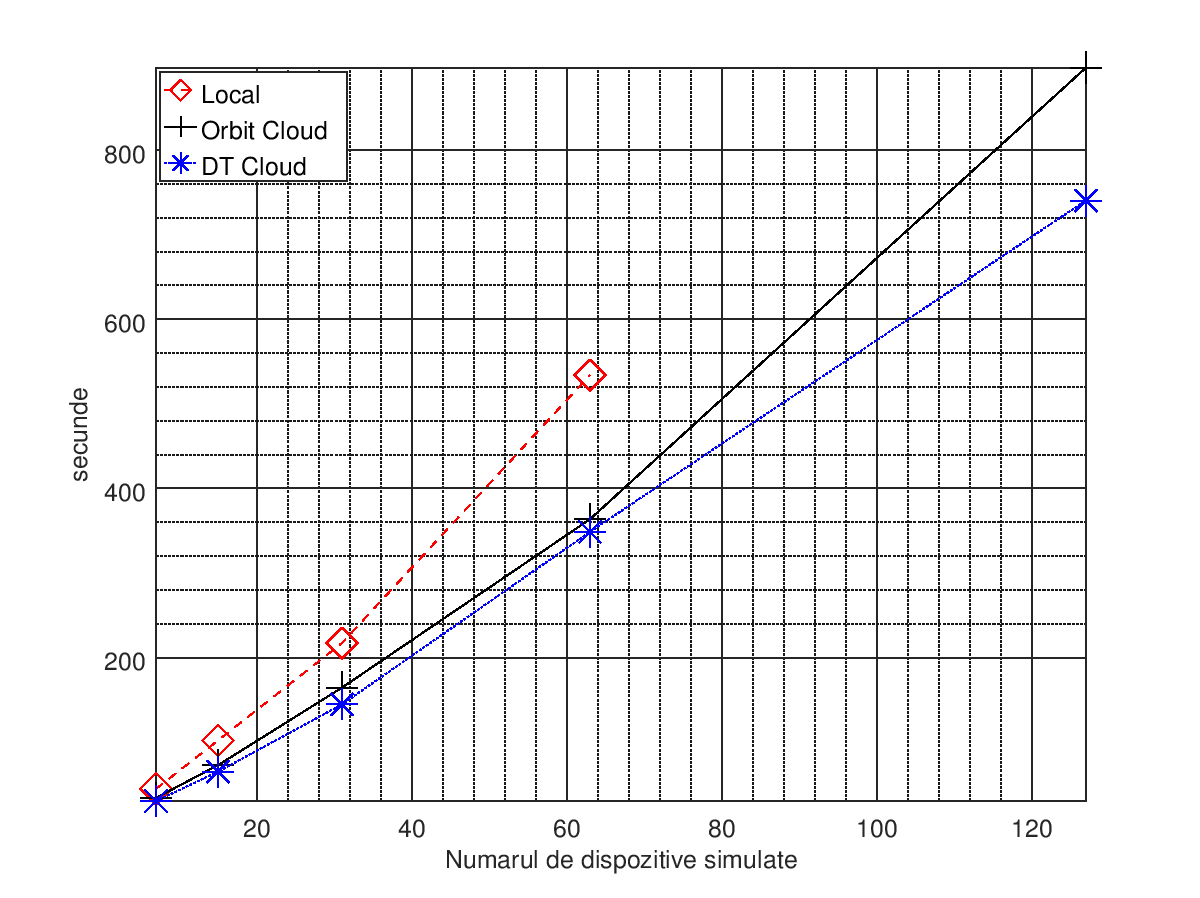
\includegraphics[width=0.85\textwidth]{boot_vs_ne_tree_v1}
	\caption{Timpul de iniţializare în funcție de numărul de dispozitive de rețea simulate, într-o rețea de tip \textbf{arbore}}
	\label{fig:boot_vs_ne_tree_v1}
\end{figure}

\begin{figure}[hp]
	\centering
	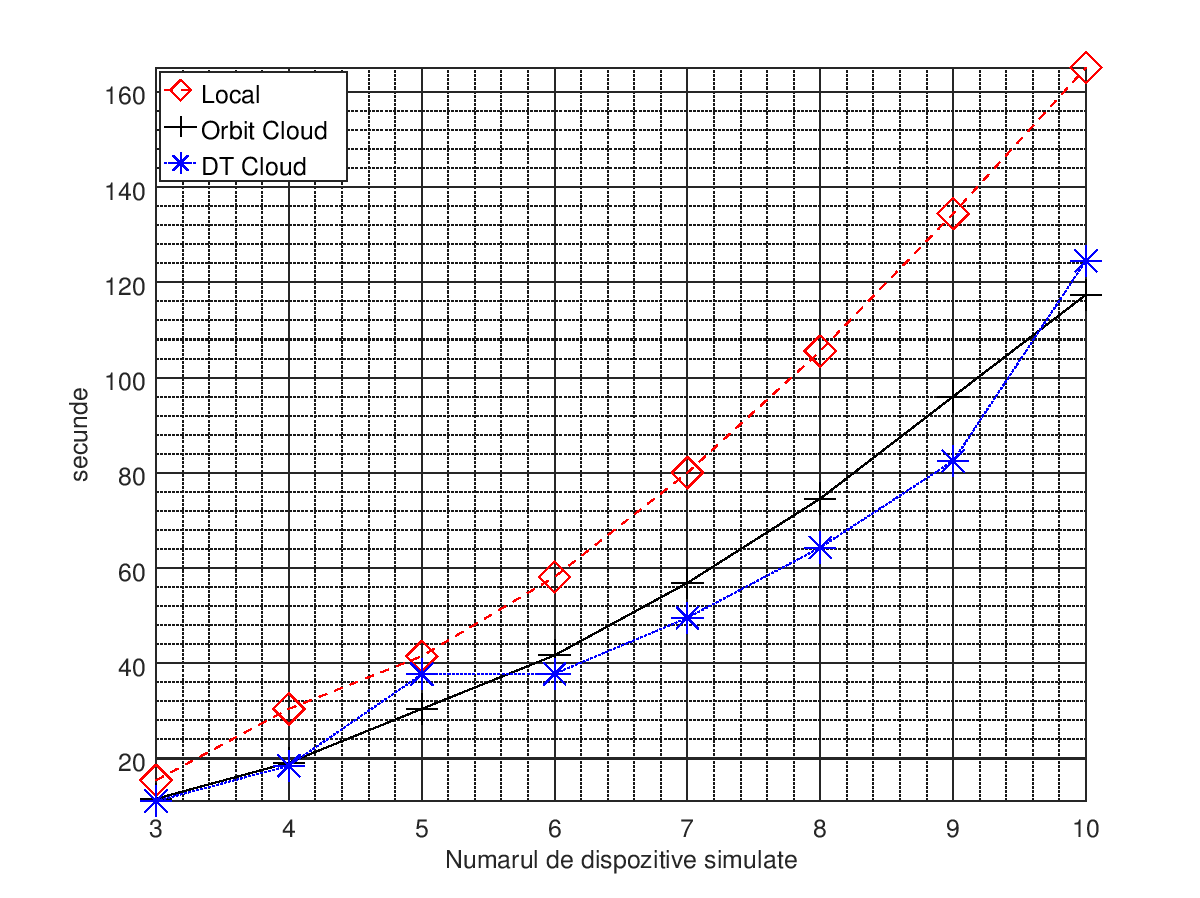
\includegraphics[width=0.85\textwidth]{boot_vs_ne_mesh_v1}
	\caption{Timpul de iniţializare în funcție de numărul de dispozitive de rețea simulate, într-o rețea de tip \textbf{plasă}}
	\label{fig:boot_vs_ne_mesh_v1}
\end{figure}

Se poate observa că, deşi frecvenţa procesorului în cazul măsurătorilor locale este mai mare decât cea a procesoarelor din mediile de tip \textit{cloud}, din cauza faptului că există două niveluri de virtualizare (unul dat de maşina virtuală Linux, celălalt de containerele \textit{docker}), iniţializarea în mediul de simulare local este mai lentă decât în celelalte cazuri (unde există un singur nivel de virtualizare). Deoarece rețelele de tip inel conţin cele mai multe eşantioane pentru numărul de dispozitive simulate, variaţia liniară a timpului de iniţializare se poate observa mai clar decât în celelalte cazuri.

O altă observaţie este că acest timp este foarte mare. În cazul simulării unor topologii mari, de peste 100 de elemente, timpul de iniţializare trece de 600 de secunde, depăşind chiar 1000 de secunde pentru 200 de elemente. Acest lucru a condus la investigarea cauzei pentru care \gls{wte} porneşte atât de greu. Din cauza utilitarului \textit{docker}, toate operaţiile se fac secvenţial. Întâi se crează și pornesc containere \textit{docker} asociate cu dispozitivele de rețea simulate, după care se adaugă legăturile dintre ele și apoi restul interfeţelor, pe rând, în fiecare container. Pentru adăugarea acestor interfețe Linux în fiecare container \textit{docker}, nucleul \gls{wte} îi trimite o comandă care se rulează în interiorul acestuia, după execuţia acesteia îi trimite comanda asociată următoarei interfețe, ș.a.m.d.

Această observaţie a dus la găsirea și implementarea unei soluții care să eficientizeze acest proces de pornire a simulatorului. Deoarece utilitarul \textit{docker} nu permite execuţia de comenzi în paralel, chiar dacă elementele simulate folosesc containere diferite, nu este posibilă paralelizarea operaţiilor, chiar dacă procesorul dispune de mai multe nuclee. Soluția care a fost implementată a fost de a adăuga toate comenzile care adaugă interfețe Linux într-un container \textit{docker} într-un fişier, care apoi va fi executat. În acest mod, toate apelurile către containerul \textit{docker} prin care se adăugau interfeţele Linux se înlocuiesc cu unul singur, prin care se adaugă toate interfeţele. Timpul de iniţializare al \gls{wte} se reduce astfel semnificativ, cu până la 35\%. Aceste noi durate de pornire a simulatorului sunt ilustrate în Figurile~\ref{fig:boot_vs_ne_ring_v2}, \ref{fig:boot_vs_ne_tree_v2} și \ref{fig:boot_vs_ne_mesh_v2}.

\begin{figure}[hp]
	\centering
	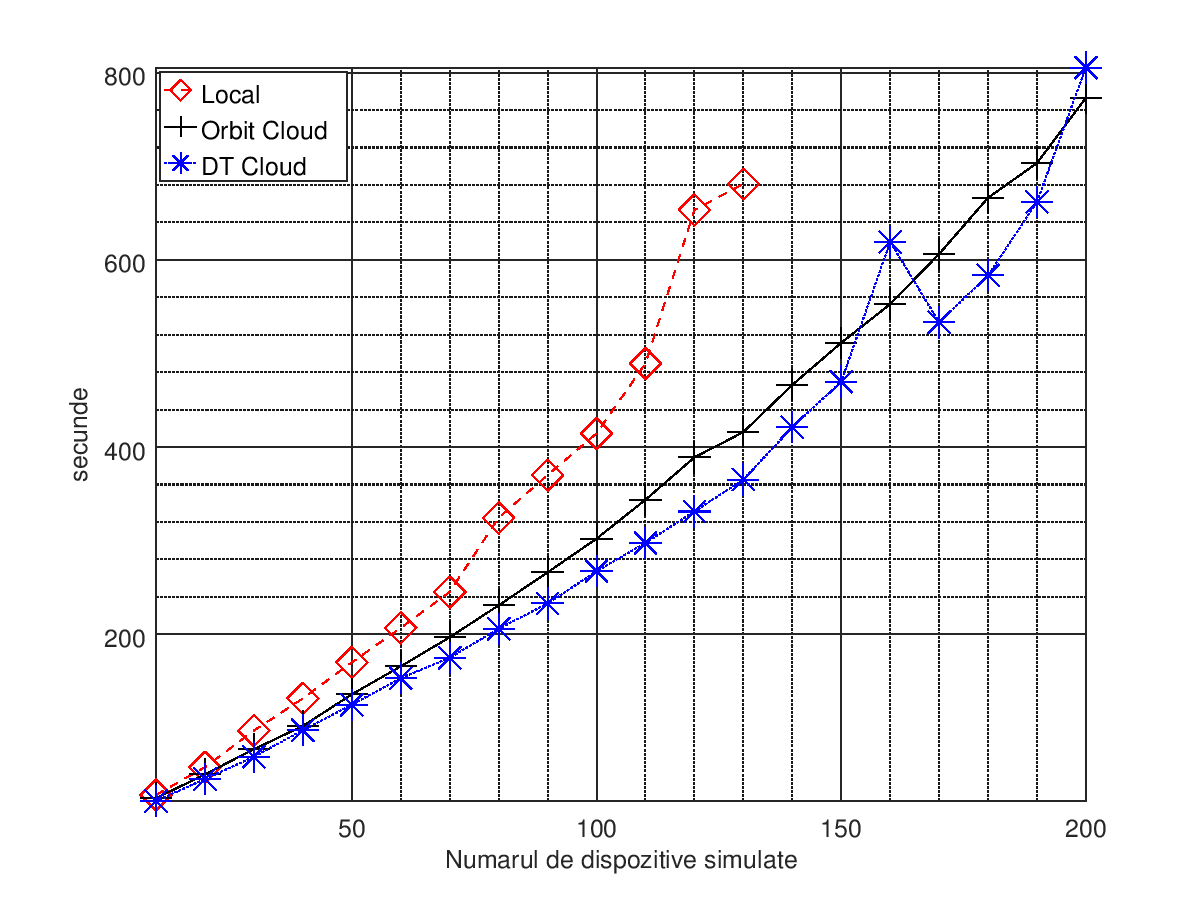
\includegraphics[width=0.85\textwidth]{boot_vs_ne_ring_v2}
	\caption{Timpul de iniţializare în funcție de numărul de dispozitive de rețea simulate, într-o rețea de tip \textbf{inel}, după optimizarea operaţiilor de pornire}
	\label{fig:boot_vs_ne_ring_v2}
\end{figure}

\begin{figure}[hp]
	\centering
	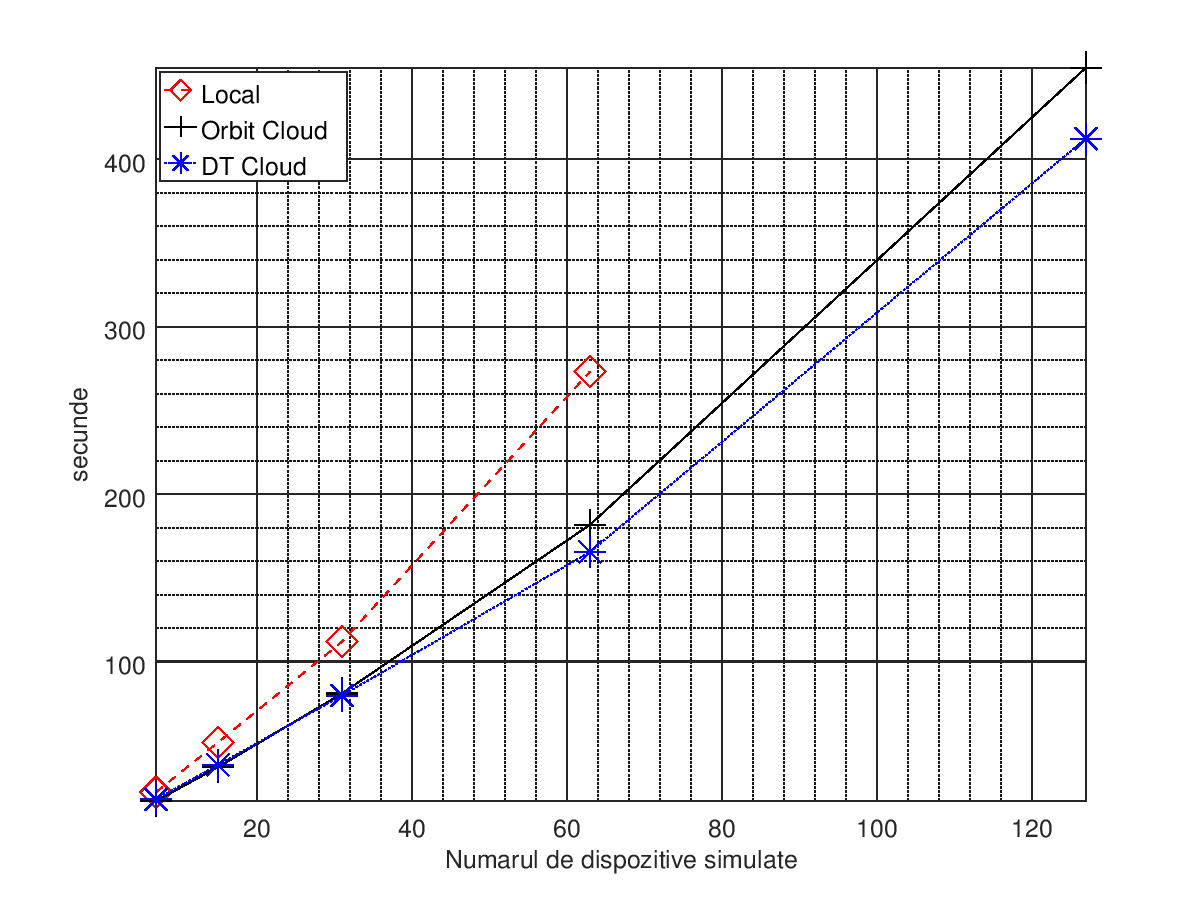
\includegraphics[width=0.85\textwidth]{boot_vs_ne_tree_v2}
	\caption{Timpul de iniţializare în funcție de numărul de dispozitive de rețea simulate, într-o rețea de tip \textbf{arbore}, după optimizarea operaţiilor de pornire}
	\label{fig:boot_vs_ne_tree_v2}
\end{figure}

\begin{figure}[hp]
	\centering
	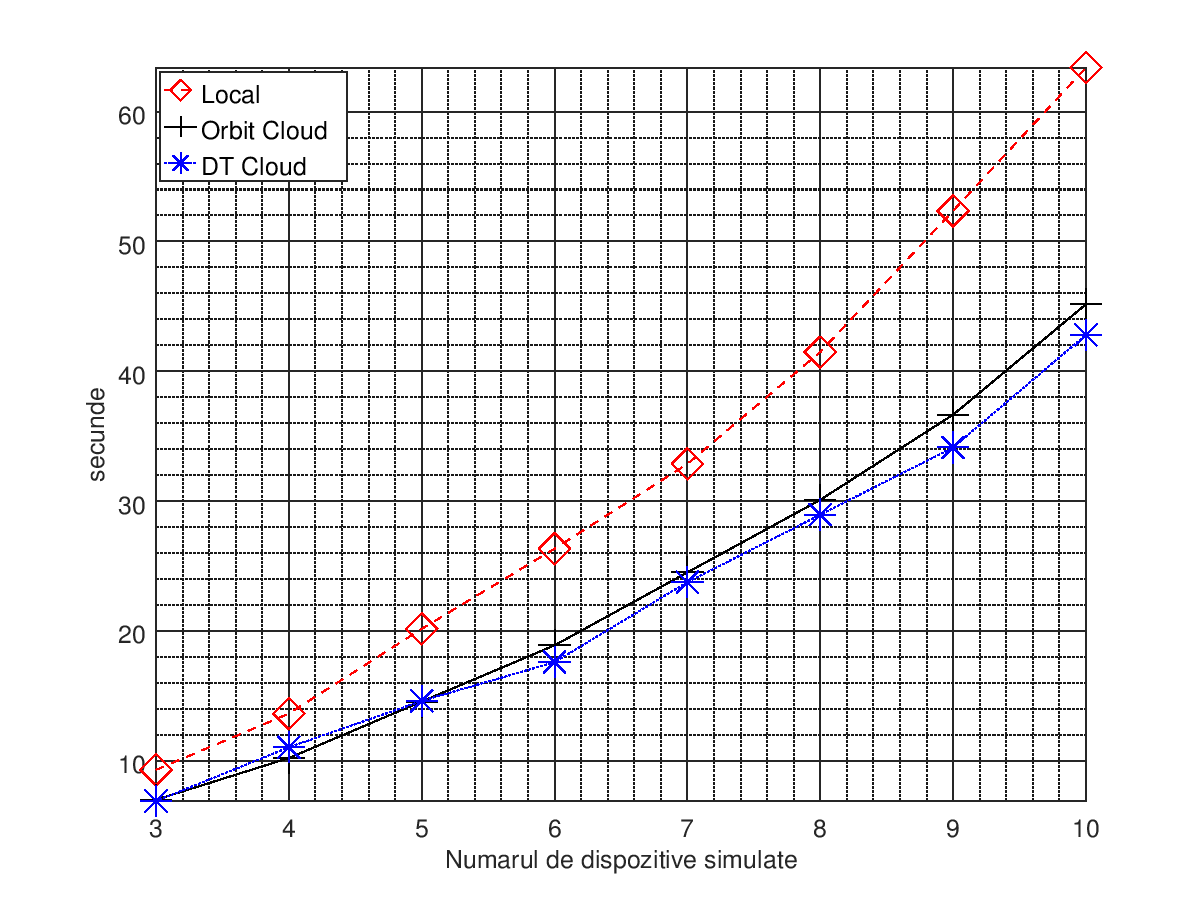
\includegraphics[width=0.85\textwidth]{boot_vs_ne_mesh_v2}
	\caption{Timpul de iniţializare în funcție de numărul de dispozitive de rețea simulate, într-o rețea de tip \textbf{plasă}, după optimizarea operaţiilor de pornire}
	\label{fig:boot_vs_ne_mesh_v2}
\end{figure}

\subsection{Spaţiul ocupat pe disc}

Următoarea caracteristică măsurată pentru \gls{wte} a fost spaţiul pe care topologiile simulate îl ocupă pe disc. Acesta este dat de utilitarul \textit{docker}, care are nevoie de el pentru reprezentarea sistemului de fişiere din interiorul fiecărui container \textit{docker}, dar și pentru salvarea informaţiilor despre interfeţele Linux reprezentate în fiecare container. Rezultatele măsurătorilor sunt ilustrate în Figurile~\ref{fig:storage_vs_ne_ring}, \ref{fig:storage_vs_ne_tree}, \ref{fig:storage_vs_ne_mesh} și \ref{fig:storage_vs_intf_mesh}.

\begin{figure}[hp]
	\centering
	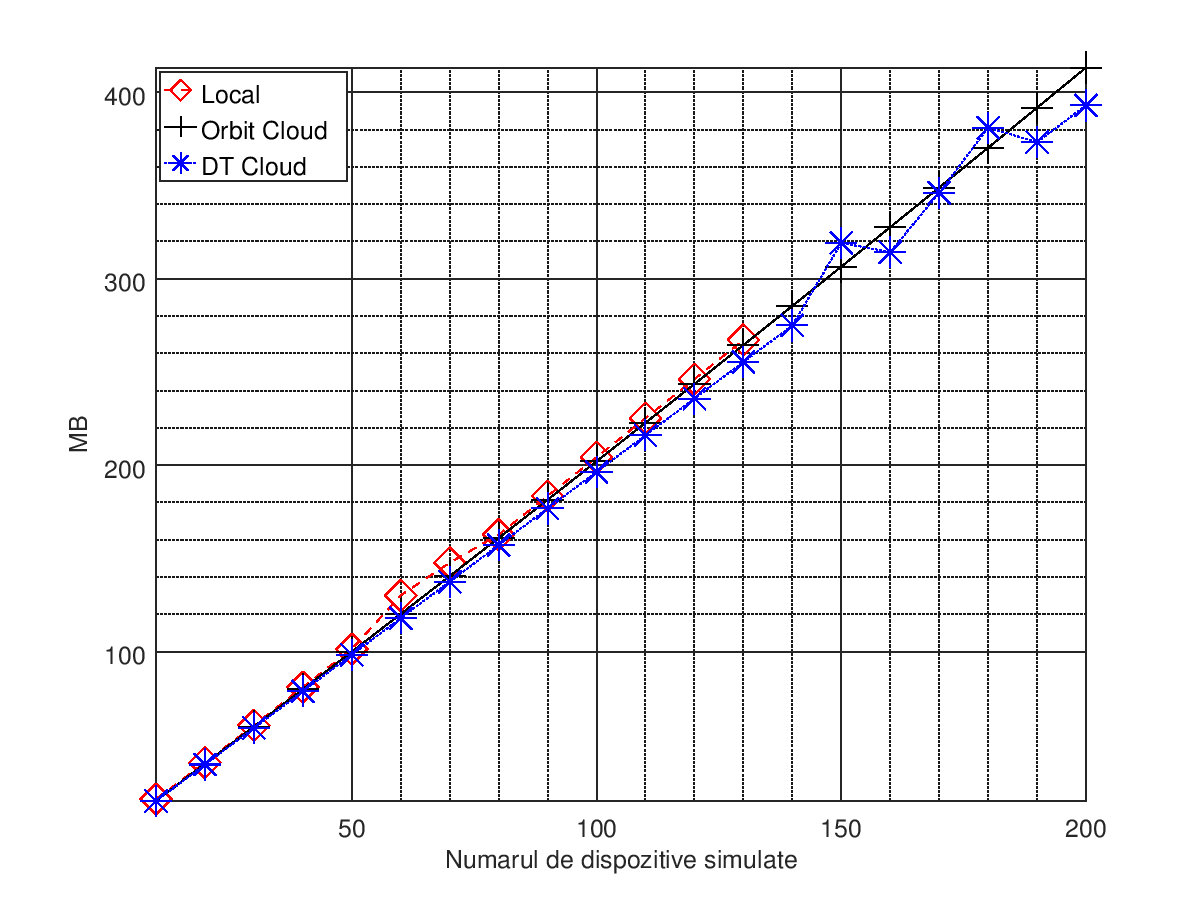
\includegraphics[width=0.85\textwidth]{storage_vs_ne_ring}
	\caption{Spaţiul de stocare utilizat în funcție de numărul de dispozitive de rețea simulate, într-o rețea de tip \textbf{inel}}
	\label{fig:storage_vs_ne_ring}
\end{figure}

\begin{figure}[hp]
	\centering
	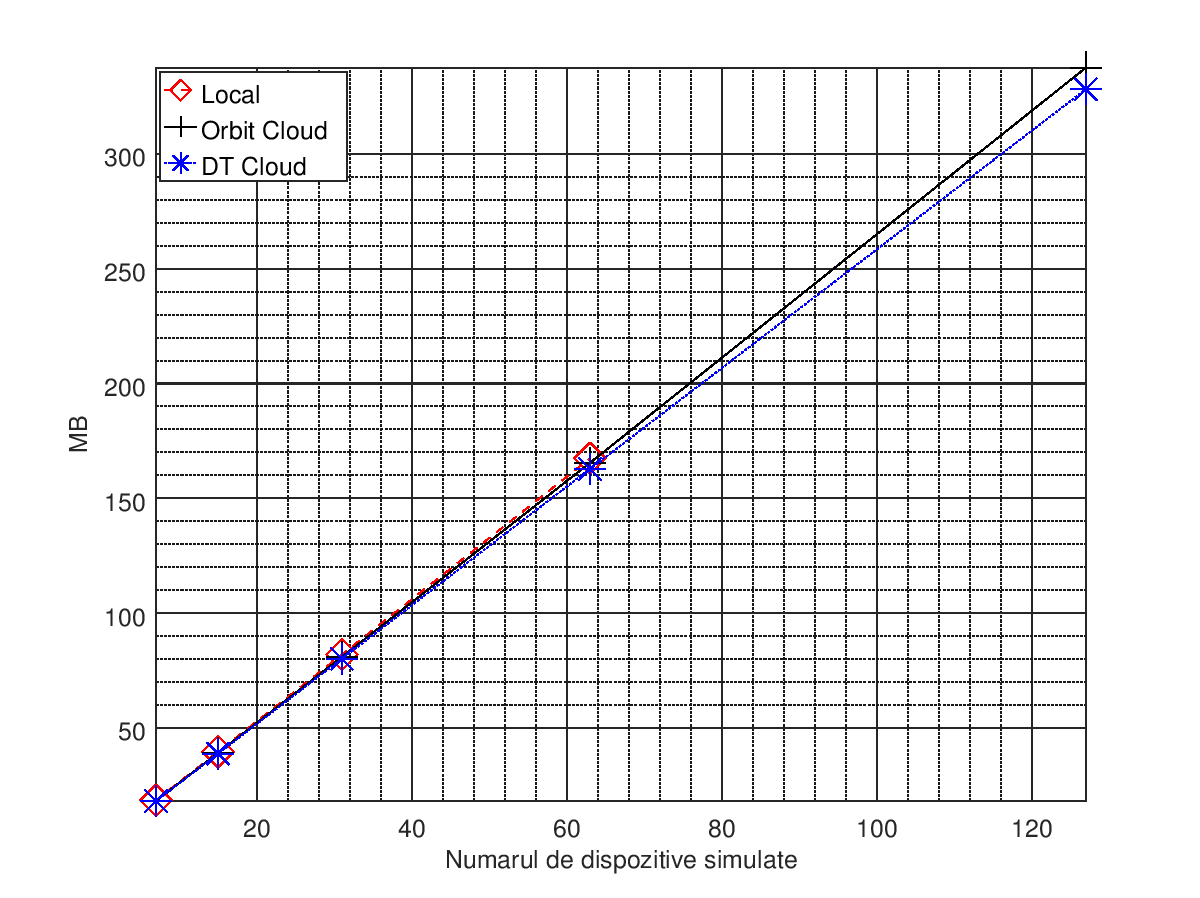
\includegraphics[width=0.85\textwidth]{storage_vs_ne_tree}
	\caption{Spaţiul de stocare utilizat în funcție de numărul de dispozitive simulate, într-o rețea de tip \textbf{arbore}}
	\label{fig:storage_vs_ne_tree}
\end{figure}

\begin{figure}[hp]
	\centering
	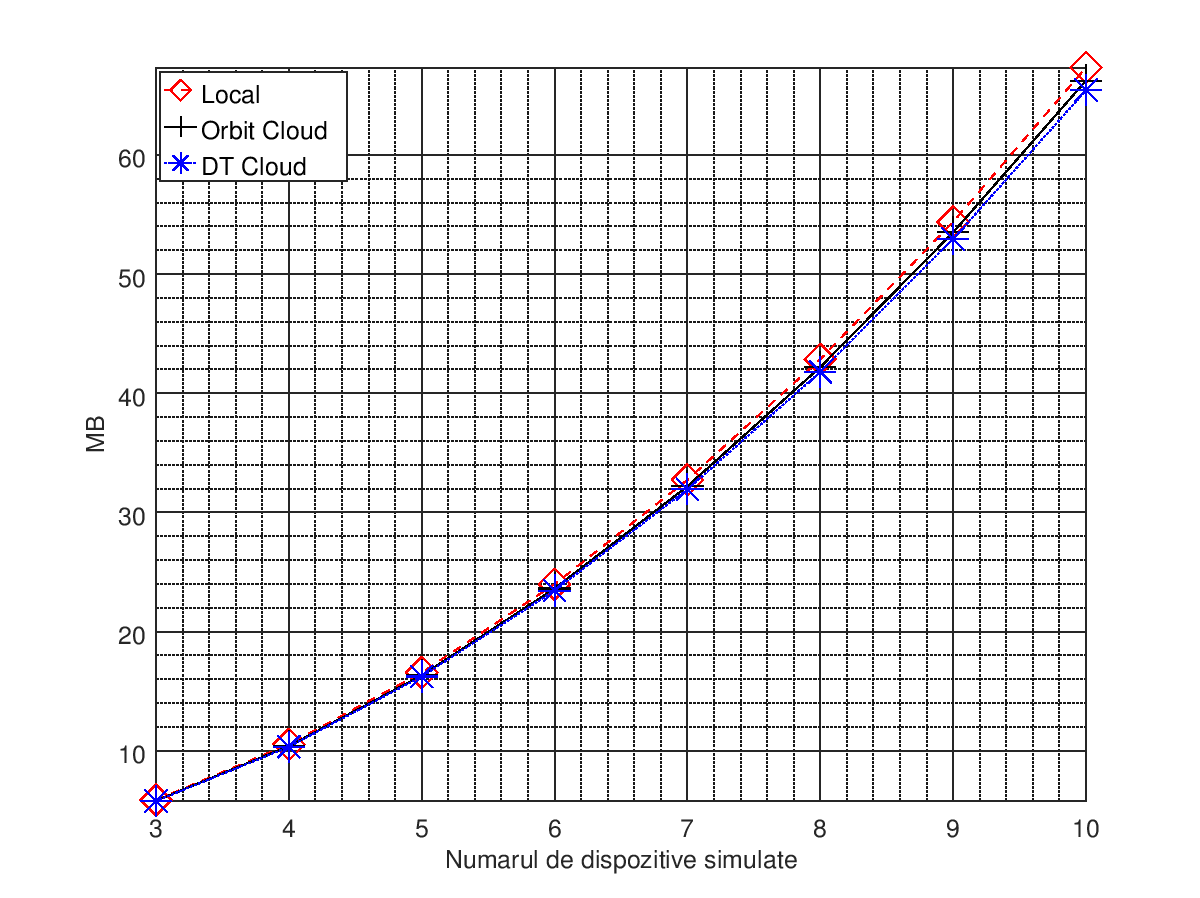
\includegraphics[width=0.85\textwidth]{storage_vs_ne_mesh}
	\caption{Spaţiul de stocare utilizat în funcție de numărul de dispozitive de rețea simulate, într-o rețea de tip \textbf{plasă}}
	\label{fig:storage_vs_ne_mesh}
\end{figure}

\begin{figure}[hp]
	\centering
	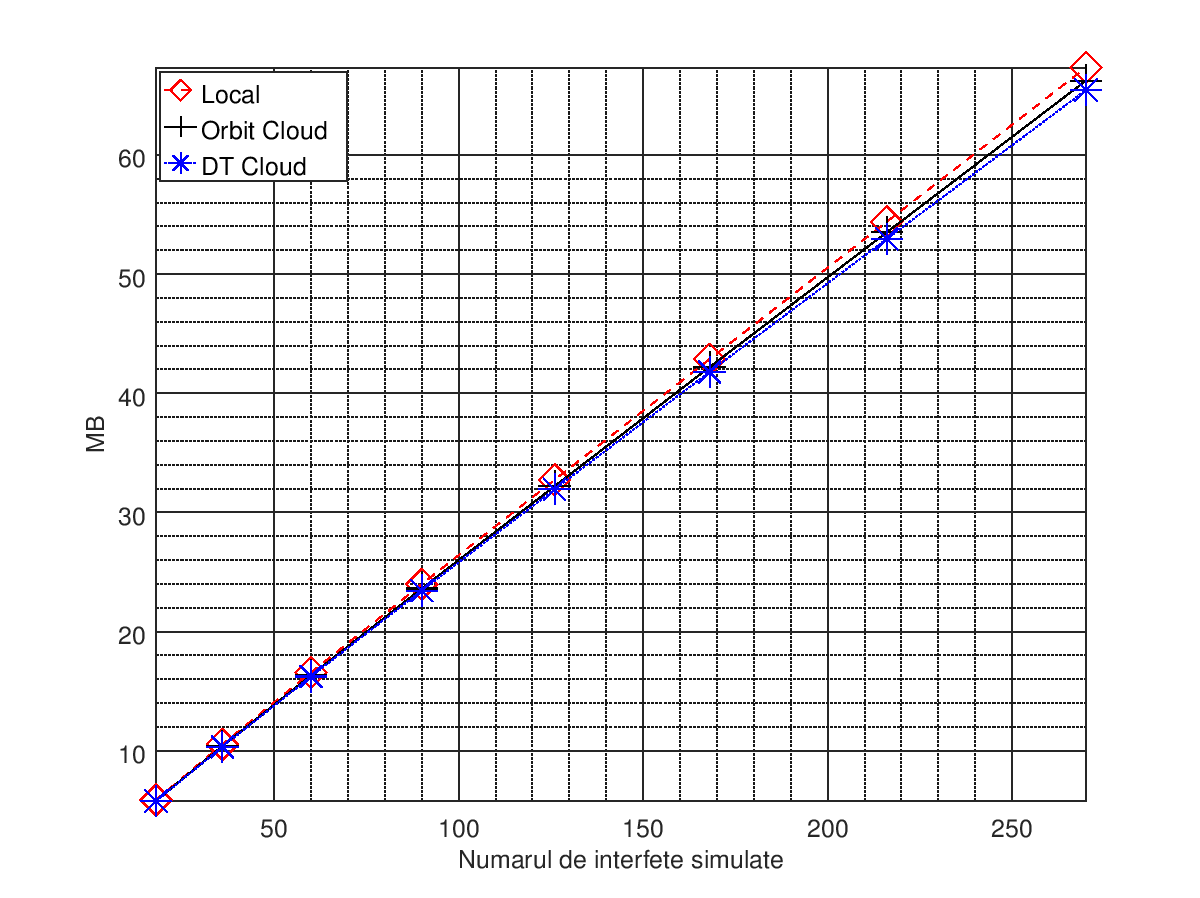
\includegraphics[width=0.85\textwidth]{storage_vs_intf_mesh}
	\caption{Spaţiul de stocare utilizat în funcție de numărul de interfețe simulate, într-o rețea de tip \textbf{plasă}}
	\label{fig:storage_vs_intf_mesh}
\end{figure}

Aceste figuri relevă faptul că spaţiul de stocare depinde liniar în principal de numărul de interfețe simulate, după cum se poate observa foarte clar în Figurile~\ref{fig:storage_vs_ne_mesh} și \ref{fig:storage_vs_intf_mesh}. În graficul ce reprezintă spaţiul de stocare în funcție de numărul de dispozitive simulate într-o topologie de tip plasă se poate observa o dependenţă pătratică, în timp ce în graficul ce prezintă spaţiul de stocare în funcție de numărul de interfețe simulate, în topologia de tip plasă, această dependenţă este liniară, de unde concluzia că această caracteristică măsurată depinde în principal de numărul interfeţelor simulate.

În cazul rețelelor de tip inel, la un număr de aproximativ 120 de dispozitive simulate, însemnând 960 de interfețe simulate, spaţiul de stocare ocupat de \gls{wte} ajunge în jurul valorii de 240 MB, pentru rețelele de tip arbore cu un număr de 120 de dispozitive simulate, adică aproximativ 1270 de interfețe simulate, sunt utilizaţi aproximativ 330 MB. Pentru rețelele de tip plasă, la un număr de 10 dispozitive simulate, având 270 de interfețe simulate, spaţiul pe disc utilizat ajunge la 65 MB. Practic, aceste valori duc la o medie aproximativă de 0,25 MB per interfață simulată.

\subsection{Puterea de procesare folosită}

Caracteristicile măsurate anterior nu sunt foarte importante după ce simulatorul a fost pornit: timpul de iniţializare nu mai e relevant, iar spaţiul de stocare nu are valori atât de mari (în funcție de topologie ajunge la zeci sau sute de MB) încât sa fie o problemă pe majoritatea maşinilor de calcul din zilele noastre. Însă, puterea de procesare și procentul memoriei cu acces aleator sunt caracteristici importante, deoarece limitează practic topologiile ce pot fi simulate pe un sistem.

Puterea de procesare măsurată este reprezentată ca procentul de folosire a procesorului, raportat la puterea totală de procesare a sistemului. De exemplu, dacă avem un procesor cu patru nuclee, iar simulatorul ar avea o putere de procesare folosită de 25\%, ar însemna că un nucleu este folosit în exclusivitate de către \gls{wte}.

Rezultatele măsurătorilor puterii de procesare folosită sunt ilustrate în Figurile~\ref{fig:cpu_vs_intf_ring}, \ref{fig:cpu_vs_intf_tree} și \ref{fig:cpu_vs_intf_mesh}.

\begin{figure}[hp]
	\centering
	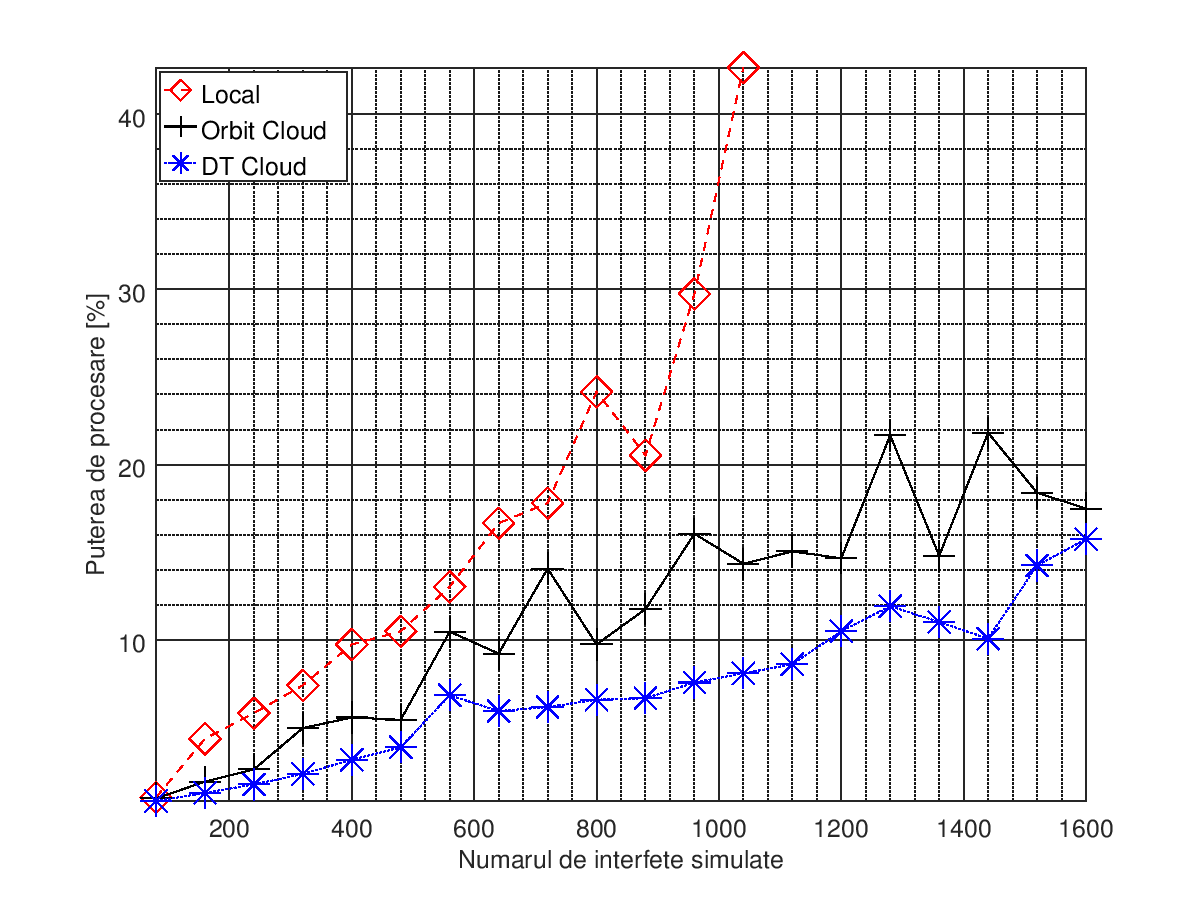
\includegraphics[width=0.85\textwidth]{cpu_vs_intf_ring}
	\caption{Puterea de procesare folosită în funcție de numărul de interfețe simulate, într-o rețea de tip \textbf{inel}}
	\label{fig:cpu_vs_intf_ring}
\end{figure}

\begin{figure}[hp]
	\centering
	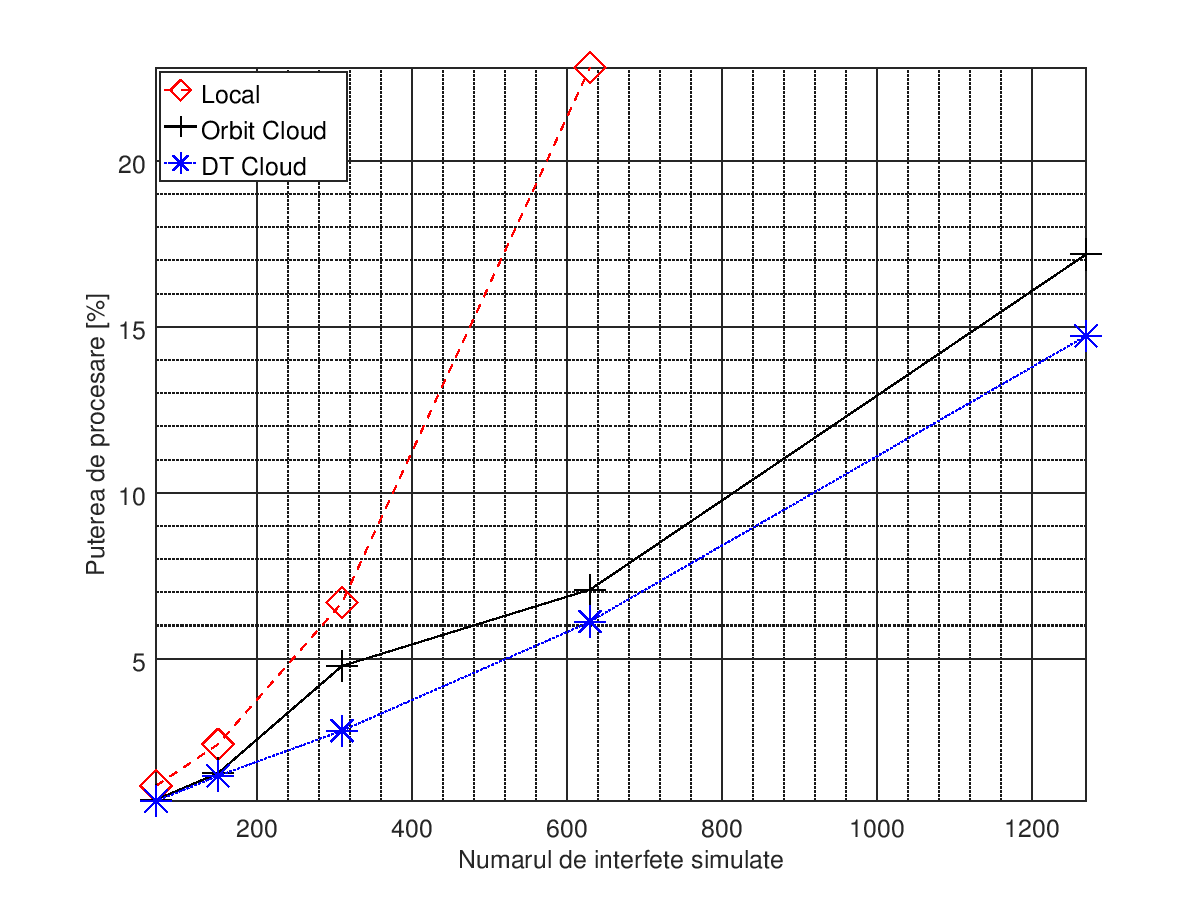
\includegraphics[width=0.85\textwidth]{cpu_vs_intf_tree}
	\caption{Puterea de procesare folosită în funcție de numărul de interfețe simulate, într-o rețea de tip \textbf{arbore}}
	\label{fig:cpu_vs_intf_tree}
\end{figure}

\begin{figure}[hp]
	\centering
	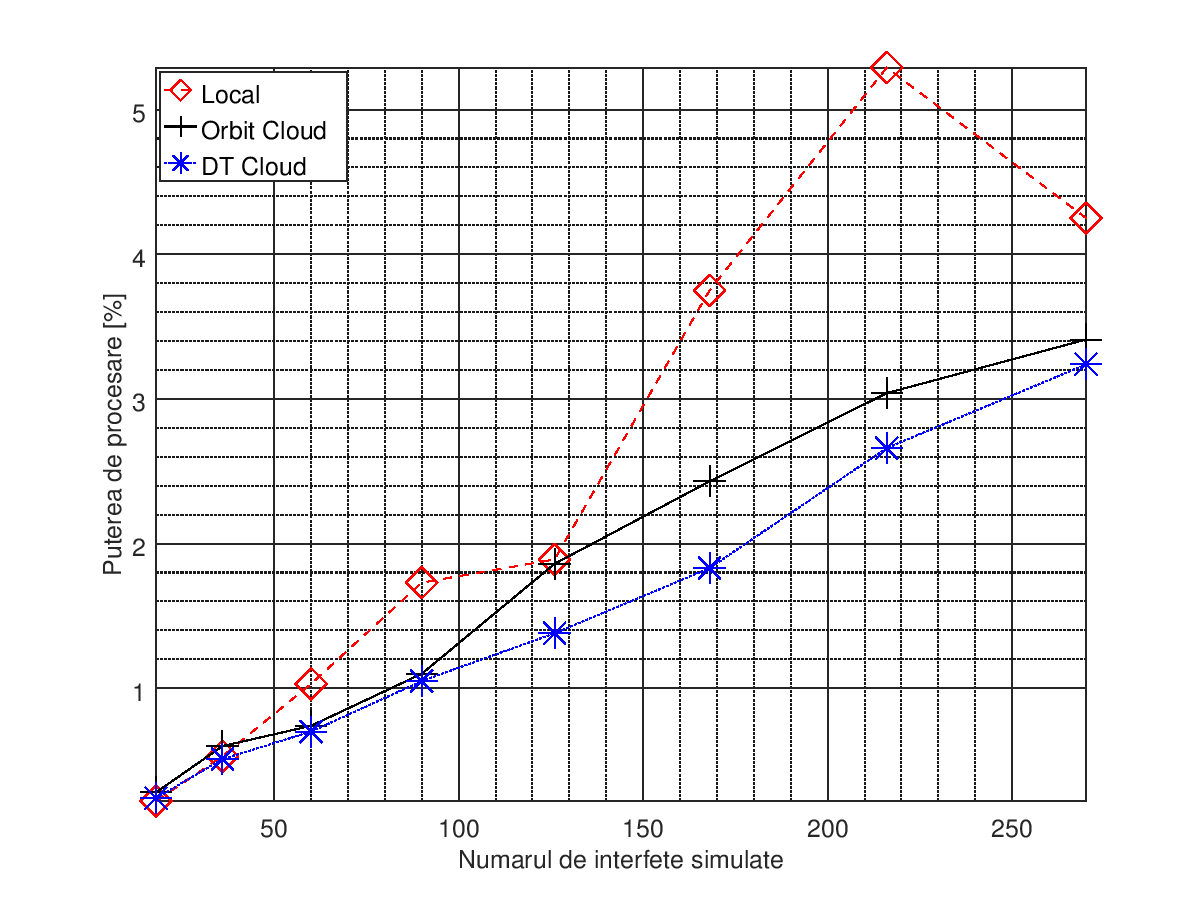
\includegraphics[width=0.85\textwidth]{cpu_vs_intf_mesh}
	\caption{Puterea de procesare folosită în funcție de numărul de interfețe simulate, într-o rețea de tip \textbf{plasă}}
	\label{fig:cpu_vs_intf_mesh}
\end{figure}

Se poate observa, cu ajutorul acestor măsurători, că puterea de procesare folosită de către \gls{wte}, chiar prin măsurarea mai multor eşantioane și calcularea unei valori medii, nu are o variaţie perfect liniară cu una dintre variabilele prezente în diferitele topologii (numărul de dispozitive, numărul de interfețe sau numărul de legături de date). Măsurătorile din cele două medii de tip \textit{cloud} (Orbit si DT) au tendinţe asemănătoare, chiar dacă variaţia puterii de procesare nu este perfect liniară cu numărul de interfețe simulate. Măsurătorile locale, însă, de la un punct, nu mai respectă această tendinţă liniară. Cel mai probabil, acest lucru este influenţat de nivelul în plus de virtualizare, dat de maşina Linux pe care este instalat mediul de simulare \gls{wte}.

Pentru un număr de 250 de interfețe simulate, în cazul topologiei de tip plasă, puterea de procesare utilizată de \gls{wte} ajunge la aproximativ 3\%, pentru un număr de 1200 de interfețe simulate, în cazul topologiei de tip inel, puterea de procesare folosită se situează în jurul valorii de 12\%, în timp ce pentru același număr de interfețe în cazul topologiei de tip arbore simulatorul utilizează aproximativ 14\% din puterea de procesare a sistemului.

Un alt scenariu a fost considerat pentru a măsura influenţa injectării de trafic în rețeaua simulată asupra puterii de procesare de care \gls{wte} are nevoie. Acesta a constat în simularea unei topologii de tip plasă cu redundanţă maximă cu 10 dispozitive, așa cum se poate observa în Figura~\ref{fig:mesh_topo_traffic}. Pentru ca figura să nu fie încărcată în mod excesiv, au fost ilustrate doar legăturile de date prin care trece traficul dintre dispozitivele de rețea.

\begin{figure}[hp]
	\centering
	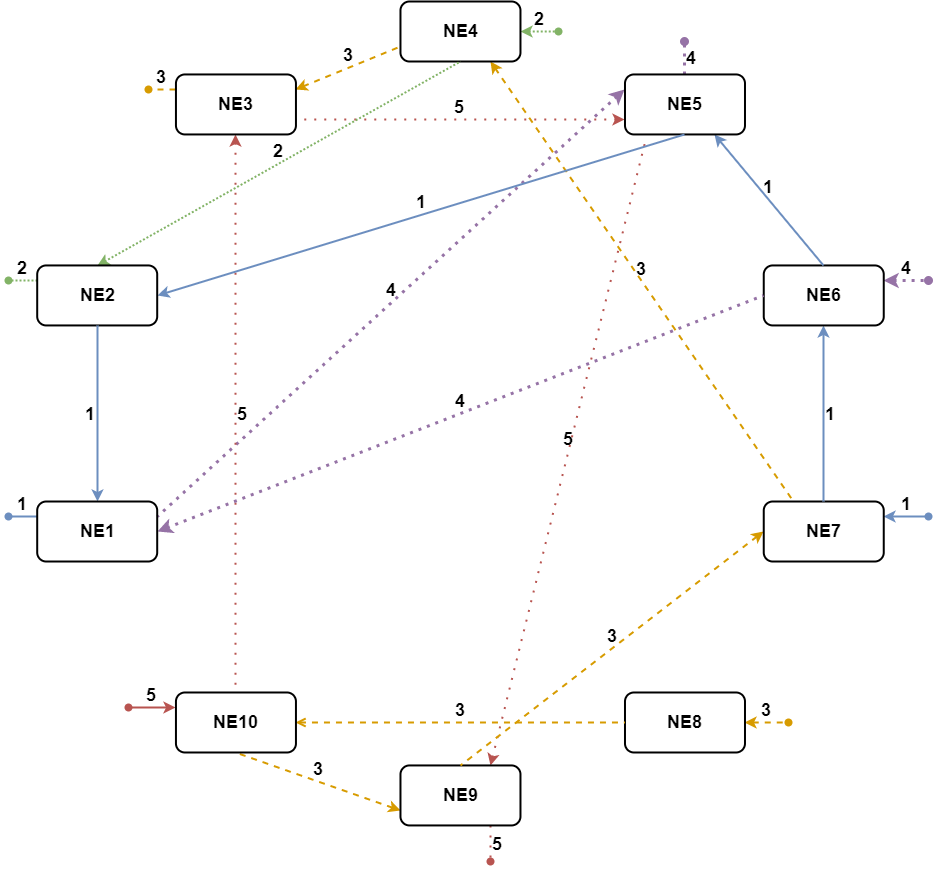
\includegraphics[width=1\textwidth]{mesh_topo_traffic}
	\caption{Topologie de tip plasă în care sunt reprezentate fluxurile de trafic simulate}
	\label{fig:mesh_topo_traffic}
\end{figure}

Primul pas a fost măsurarea puterii de procesare utilizată de topologia simulată în condiţiile în care nu era injectat niciun flux de trafic. Apoi, a fost măsurată puterea de procesare în cazul în care se folosea un flux de trafic, apoi două, până la cinci fluxuri, conform figurii anterioare.

Figura~\ref{fig:cpu_mesh_traffic} prezintă valorile cu care puterea de procesare folosită de \gls{wte} creşte față de cazul fără trafic, în funcție de numărul de fluxuri de trafic ce se transmit în paralel prin rețeaua simulată.

\begin{figure}[hp]
	\centering
	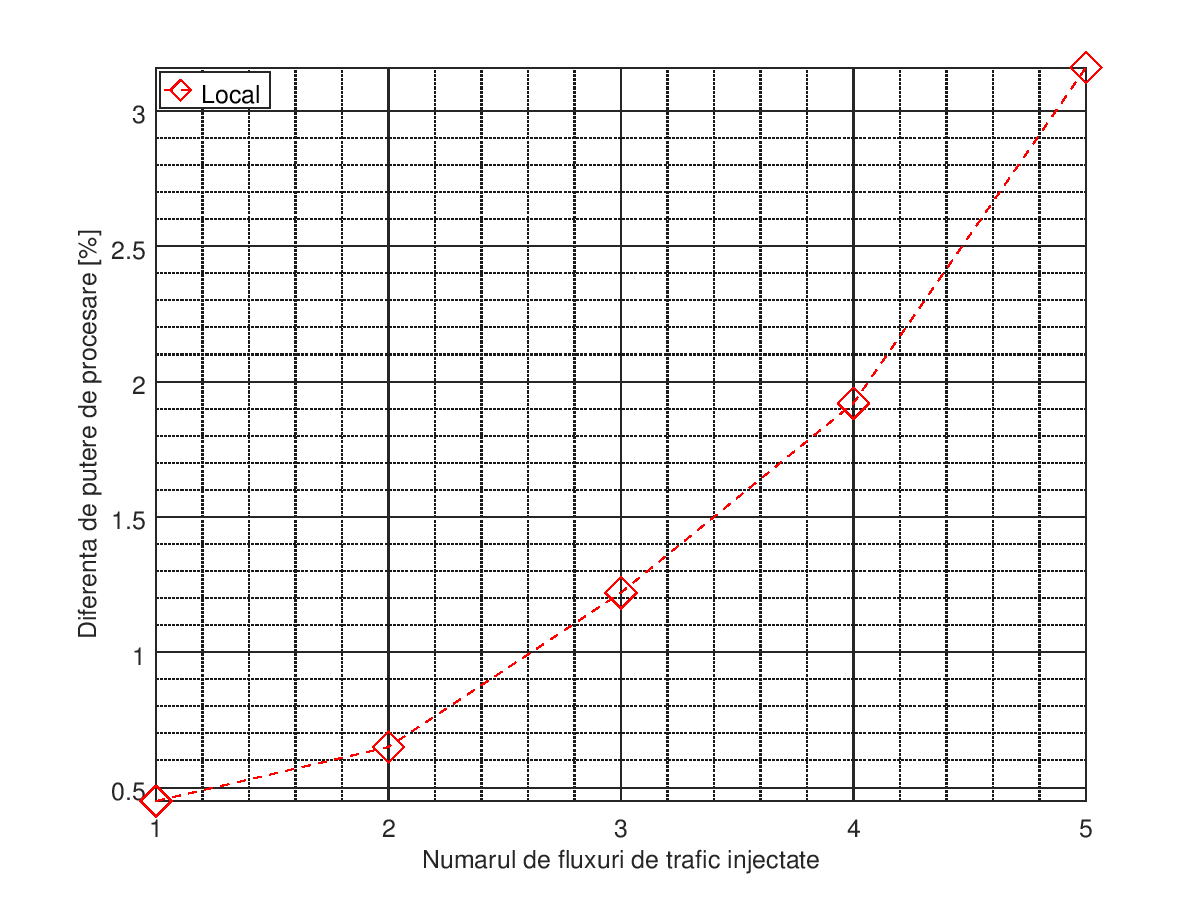
\includegraphics[width=0.8\textwidth]{cpu_mesh_traffic}
	\caption{Puterea de procesare de care injectarea de trafic are nevoie, într-o rețea de tip plasă cu redundanţă maximă, în funcție de numărul de fluxuri de trafic injectate în rețea}
	\label{fig:cpu_mesh_traffic}
\end{figure}

Putem observa că puterea de procesare folosită pentru transmiterea de trafic în rețeaua simulată creşte exponenţial cu numărul de fluxuri injectate, ajungând la 3\% pentru 5 astfel de conexiuni. Aceasta este utilizată de serverele și clienţii utilitarului \textit{iperf3} asociaţi cu aceste operații de transfer de date.

\subsection{Memoria cu acces aleator}

Ultima caracteristică măsurată pentru \gls{wte} este reprezentată de procentul de memorie cu acces aleator folosit de către simulator, raportat la totalul memoriei cu acces aleator disponibilă în sistem. Aceasta este practic cea mai importantă caracteristică folosită de \gls{wte}, care va limita de fapt numărul de dispozitive de rețea sau interfețe ce pot fi simulate. Dacă în cazul procentului de putere de procesare, în cazul în care simulatorul are nevoie de un procent mare, acestuia îi va reveni, la un moment dat și simulatorul va fi executat în continuare de către sistemul de operare, chiar dacă execuţia întregului sistem va deveni greoaie, în cazul procentului de memorie cu acces aleator, dacă \gls{wte} va mai încerca să aloce memorie și sistemul nu îi mai poate îndeplini cererea, execuţia simulatorului va fi terminată de către sistemul de operare.

Rezultatele măsurătorilor procentului de memorie cu acces aleator folosită de simulatorul \gls{wte} sunt prezentate în Figurile~\ref{fig:mem_vs_intf_ring}, \ref{fig:mem_vs_intf_tree} și \ref{fig:mem_vs_intf_mesh}.

\begin{figure}[hp]
	\centering
	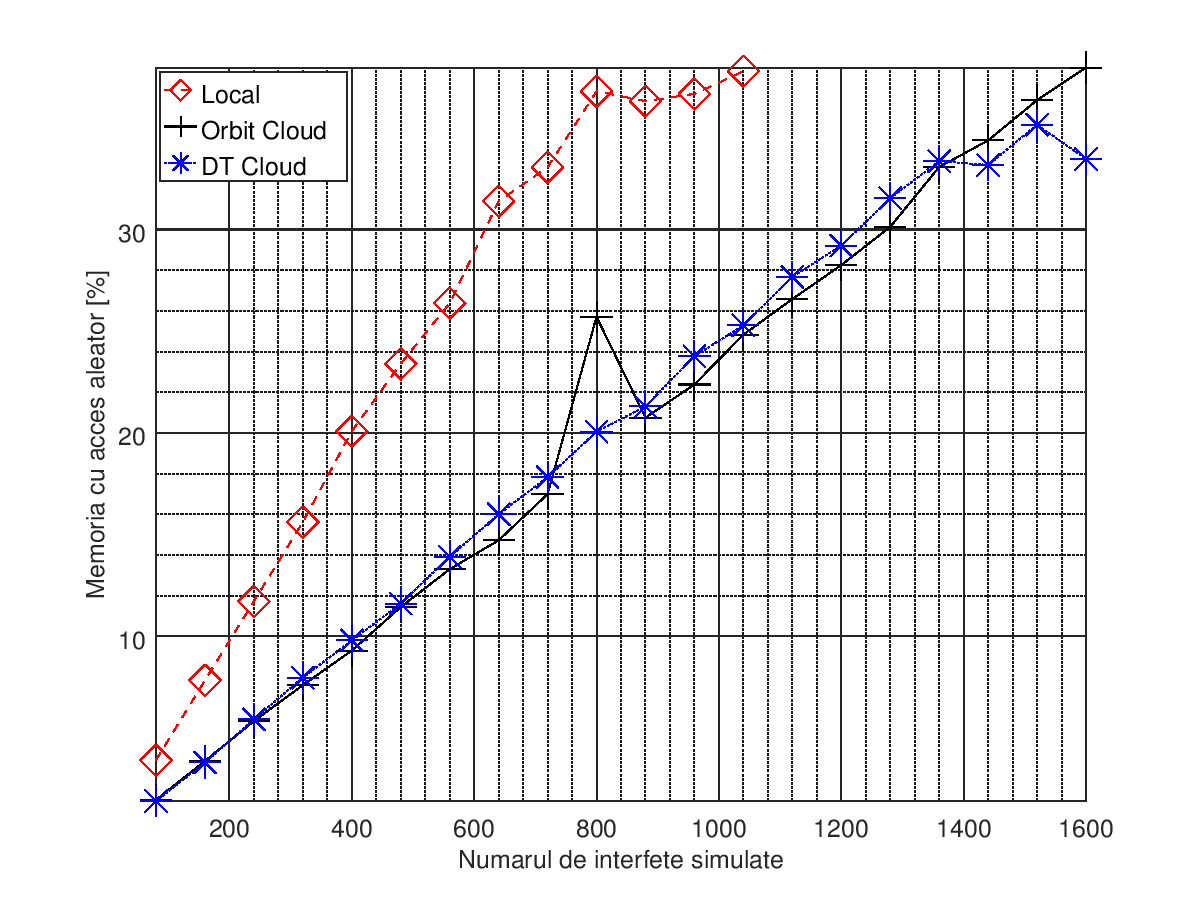
\includegraphics[width=0.85\textwidth]{mem_vs_intf_ring}
	\caption{Memoria cu acces aleator folosită în funcție de numărul de interfețe simulate, într-o rețea de tip \textbf{inel}}
	\label{fig:mem_vs_intf_ring}
\end{figure}

\begin{figure}[hp]
	\centering
	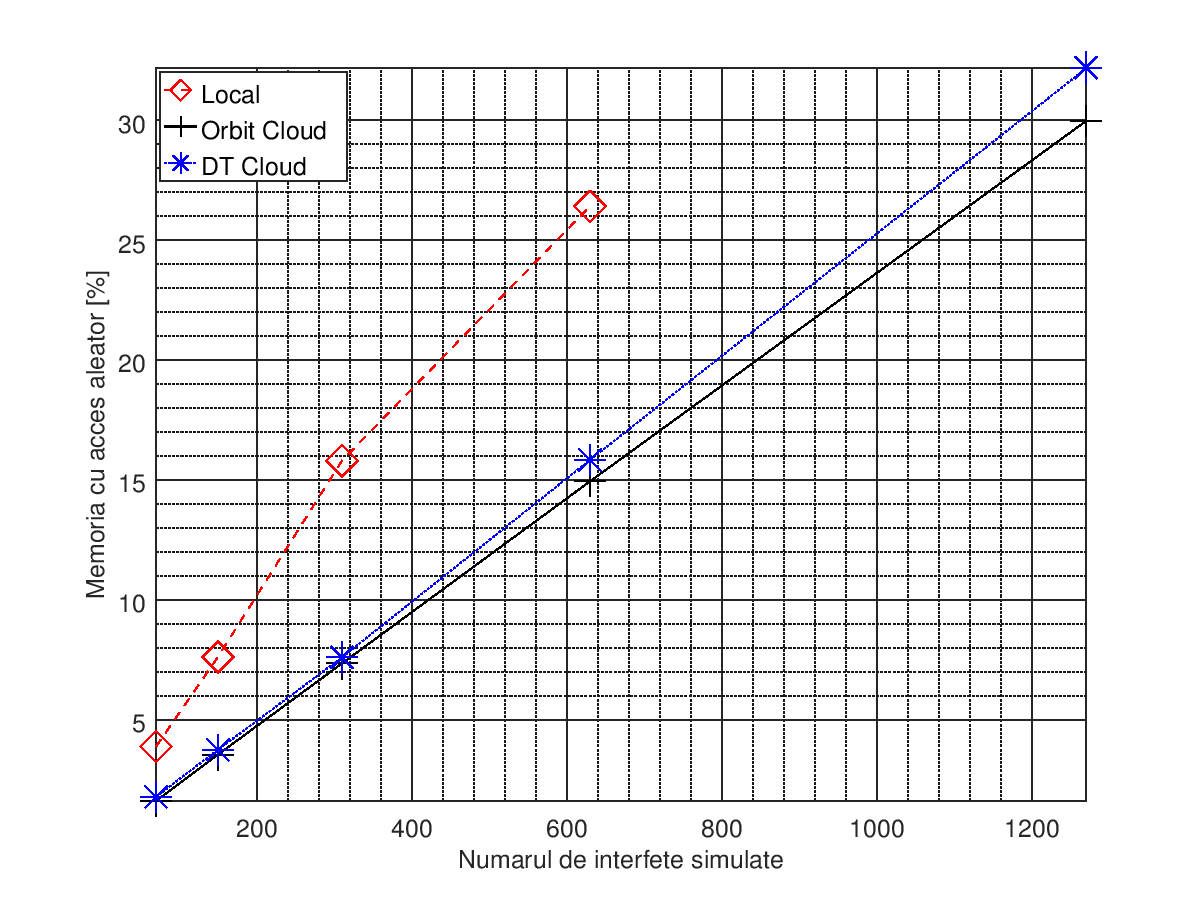
\includegraphics[width=0.85\textwidth]{mem_vs_intf_tree}
	\caption{Memoria cu acces aleator folosită în funcție de numărul de interfețe simulate, într-o rețea de tip \textbf{arbore}}
	\label{fig:mem_vs_intf_tree}
\end{figure}

\begin{figure}[hp]
	\centering
	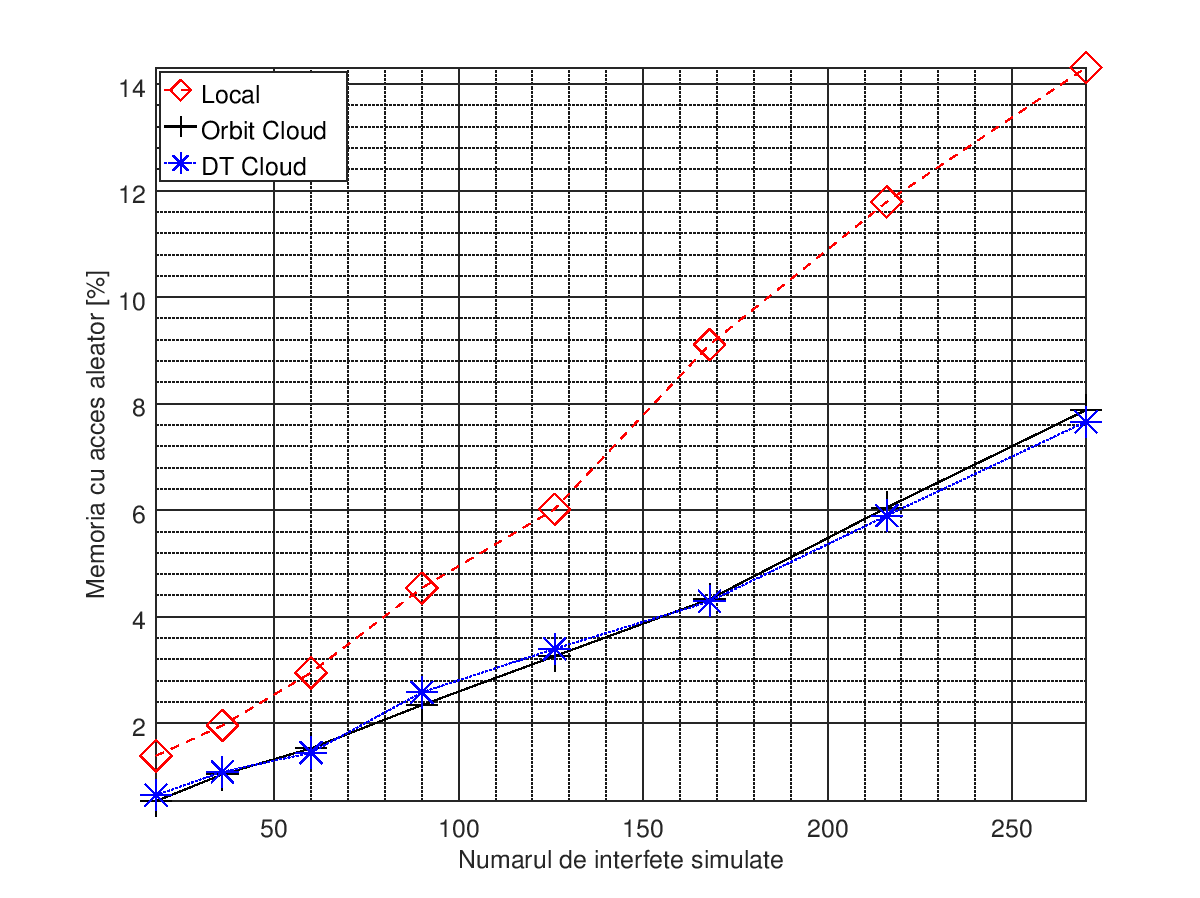
\includegraphics[width=0.85\textwidth]{mem_vs_intf_mesh}
	\caption{Memoria cu acces aleator folosită în funcție de numărul de interfețe simulate, într-o rețea de tip \textbf{plasă}}
	\label{fig:mem_vs_intf_mesh}
\end{figure}

Se observă o dependenţă liniară între numărul de interfețe simulate și procentul de memorie cu acces aleator folosită de \gls{wte}. În exemplele următoare considerăm mediile de simulare de tip \textit{cloud}, care au 8 GB de memorie cu acces aleator. Pentru topologia de tip plasă, la un număr de 200 de interfețe simulate, procentul de memorie cu acces aleator utilizat de simulator ajunge la aproximativ 5\%. Pentru topologia arbore, la 1000 de interfețe simulate, valoarea procentului de memorie cu acces aleator ajunge la aproximativ 24\%, iar în cazul topologiei de tip inel, pentru același număr de interfețe, această valoare ajunge tot în jurul pragului de 24\%. Putem concluziona astfel că, indiferent de topologia simulată, \gls{wte} are nevoie de aproximativ 0,025\% memorie cu acces aleator pentru fiecare interfață pe care o va simula, adică 2 MB, având în vedere că am considerat cazul în care sistemul dispune de un total de 8 GB.

\subsection{Concluziile evaluării}

Rezultatele evaluării ilustrează câteva concluzii interesante despre \gls{wte}. Variabila care influenţează cel mai mult comportamentul simulatorului nu este numărul de dispozitive de rețea simulate, așa cum poate era de așteptat, ci numărul de interfețe pe care topologia le conţine. Cu cât acest număr este mai mare, cu atât timpul de iniţializare a simulatorului, memoria cu acces aleator utilizată și spaţiul pe disc necesar sunt mai mari.

Timpul de iniţializare a simulatorului este destul de mare în cazul topologiilor mari, ajungând la sute de secunde pentru rețele care conţin mii de interfețe. Acest timp nu este critic pentru funcționarea \gls{wte}, deoarece, odată pornit, simulatorul nu mai are nevoie să fie redeschis decât în cazul în care se doreşte schimbarea topologiei simulate. Influenţează, însă, experienţa de folosire pe care o are utilizatorul. După ce s-a optimizat iniţializarea \gls{wte} prin gruparea creării interfeţelor Linux asociate obiectelor \gls{ltp}, timpul de iniţializare a fost îmbunătăţit semnificativ, dar este influenţat în continuare în principal de durata creării și pornirii containerelor \textit{docker} asociate dispozitivelor de rețea simulate. Acest timp nu poate fi îmbunătăţit, deoarece utilitarul \textit{docker} nu permite paralelizarea acestor operații.

Spaţiul de stocare pe disc nu pare să reprezinte o problemă în folosirea \gls{wte}, chiar și în cazul simulării unor topologii de rețea foarte mari. Acesta depinde de numărul de interfețe, simulatorul având nevoie de aproximativ 0,25 MB pentru fiecare interfață simulată. Astfel, pentru o rețea ce conţine 4000 de interfețe, \gls{wte} va folosi aproximativ 1 GB de memorie pe disc, ceea ce nu reprezintă o problemă pentru majoritatea sistemelor din zilele noastre.

Memoria cu acces aleator necesară pentru execuţia \gls{wte} prezintă o dependenţă liniară de numărul de interfețe simulate. Conform rezultatelor prezentate anterior, indiferent de tipul de topologie care este simulată, \gls{wte} are nevoie de aproximativ 2 MB de memorie cu acces aleator pentru fiecare interfață care trebuie reprezentată.

Puterea de procesare este caracteristica simulatorului care variază cel mai mult și cel mai puţin predictibil. Observăm o creștere a acesteia cu numărul de dispozitive de rețea simulate, cu numărul de interfețe dar și cu numărul de fluxuri de trafic ce se injectează în rețea. Această caracteristică nu este predictibilă, deoarece utilitarul \textit{docker} este responsabil de alocarea de putere de procesare fiecărui container, în funcție de nevoile acestuia. În timpul execuţiei, aceste nevoi pot varia și în funcție de aplicațiile din echipamentul de control \gls{sdn} care administrează rețeaua.

Dimensiunea topologiilor ce pot fi simulate este dată astfel, în principal, de cantitatea de memorie cu acces aleator care este disponibilă pe sistemul unde a fost instalat mediul de simulare. În cazul unui sistem cu 4 GB de astfel de memorie, pot fi simulate până la 1000 de interfețe. Chiar dacă, conform măsurătorilor efectuate anterior, aceste 1000 de interfețe ar ocupa doar 2 GB din memoria cu acces aleator a sistemului, nu se poate folosi mai multă memorie, deoarece aceasta este folosită și de sistemul de operare și de alte eventuale aplicații care sunt executate în sistem. Pentru sisteme mai capabile, cu 8 GB de memorie cu acces aleator, numărul interfeţelor simulate poate depăşi 2500. Acestea se referă la interfeţele Linux asociate obiectelor \gls{ltp} din modelele informaționale propuse de \gls{onf}. Dacă ne referim doar la interfeţele de rețea prin care se fac legături în topologiile simulate, având în vedere că o astfel de interfață (de tip \gls{mwps}) are asociate încă două obiecte (de tip \gls{mws} și \gls{etc}), atunci putem afirma că se pot simula aproximativ 800 de astfel de interfețe.

Cu ajutorul acestei evaluări, a fost demonstrat că \gls{wte} poate reprezenta o soluție viabilă pentru dezvoltatorii de aplicații \gls{sdn}. Acesta permite simularea unor topologii diverse, care, în funcție de capabilitățile sistemului pe care este instalat, pot fi destul de mari, ajungând să conţină mii de interfețe de rețea. Astfel, dezvoltatorii pot executa și teste de extensibilitate pentru aplicațiile pe care le implementează. Chiar dacă rețelele reale, de producție, pot conţine mii de elemente și zeci de mii de interfețe, \gls{wte} este un prim pas pentru simularea unor astfel de rețele de transport de date fără fir, în contextul \gls{sdn}. În viitor, acest simulator se poate optimiza, astfel încât să permită reprezentarea unor astfel de rețele, la scara la care există în producție, sau se poate căuta o soluție în care \gls{wte} să fie executat în mod distribuit, pe mai multe sisteme.